%
%===============>>  Киселев Модуль 6 <<=============
%
\setmodule{6}

%BEGIN_FOLD % ====>>_____ Занятие 1 _____<<====
\begin{class}[number=1]
	\begin{listofex}
		\item Вычислить:
		\begin{tasks}(1)
			\task \( \dfrac{\left( 7\dfrac{1}{3} \right)^2-\left( 2\dfrac{2}{3} \right)^2}{\left( 5\dfrac{7}{9} \right)^2-\left( 4\dfrac{2}{9} \right)^2} \)
			\task \( \dfrac{42,5904:6,08-1,245}{(18,2^2-5,6^2+23,8\cdot7,4):5,95+35,2} \)
		\end{tasks}
		\item В фирме такси в наличии \( 50 \) легковых автомобилей; \( 27 \) из них чёрного цвета с жёлтыми надписями на бортах, остальные --- жёлтого цвета с чёрными надписями. Найдите вероятность того, что на случайный вызов приедет машина жёлтого цвета с чёрными надписями.
		\item Перед началом первого тура чемпионата по бадминтону участников разбивают на игровые пары случайным образом с помощью жребия. Всего в чемпионате участвует \( 26 \) бадминтонистов, среди которых \( 16 \) спортсменов из России, в том числе Тарас Селезнёв. Найдите вероятность того, что в первом туре Тарас Селезнёв будет играть с каким-либо бадминтонистом из России.
		\item В кармане у Саши было четыре конфеты --- «Маска», «Василёк», «Взлётная» и «Коровка», а так же ключи от квартиры. Вынимая ключи, Саша случайно выронил из кармана одну конфету. Найдите вероятность того, что потерялась конфета «Василёк».
		\item Какова вероятность того, что случайно выбранный телефонный номер оканчивается двумя чётными цифрами?
		\item Из районного центра в деревню ежедневно ходит автобус. Вероятность того, что в понедельник в автобусе окажется меньше \( 18 \) пассажиров, равна \( 0,82 \). Вероятность того, что окажется меньше \( 10 \) пассажиров, равна \( 0,51 \). Найдите вероятность того, что число пассажиров будет от \( 10 \) до \( 17 \).
		\item Вероятность того, что новый электрический чайник прослужит больше года, равна \( 0,97 \). Вероятность того, что он прослужит больше двух лет, равна \( 0,89 \). Найдите вероятность того, что он прослужит меньше двух лет, но больше года.
		\item Биатлонист пять раз стреляет по мишеням. Вероятность попадания в мишень при одном выстреле равна \( 0,8 \). Найдите вероятность того, что биатлонист первые три раза попал в мишени, а последние два промахнулся. Результат округлите до сотых.
		\item В магазине три продавца. Каждый из них занят с клиентом с вероятностью \( 0,3 \). Найдите вероятность того, что в случайный момент времени все три продавца заняты одновременно (считайте, что клиенты заходят независимо друг от друга).
		\item На экзамене по геометрии школьник отвечает на один вопрос из списка экзаменационных вопросов. Вероятность того, что это вопрос по теме «Вписанная окружность», равна \( 0,2 \). Вероятность того, что это вопрос по теме «Параллелограмм», равна \( 0,15 \). Вопросов, которые одновременно относятся к этим двум темам, нет. Найдите вероятность того, что на экзамене школьнику достанется вопрос по одной из этих двух тем.
		\item Два велосипедиста одновременно отправились в \( 154 \)-километровый пробег. Первый ехал со скоростью, на \( 3 \) км/ч большей, чем скорость второго, и прибыл к финишу на \( 3 \) часа раньше второго. Найти скорость велосипедиста, пришедшего к финишу вторым. Ответ дайте в км/ч. 
		
	\end{listofex}
\end{class}
%END_FOLD

%BEGIN_FOLD % ====>>_____ Занятие 2 _____<<====
\begin{class}[number=2]
	\begin{listofex}
		\item Вычислите:
		\begin{tasks}(1)
			\task \( \left( \dfrac{3}{4}+\dfrac{1}{6} \right)\cdot3+\left( \dfrac{5}{6}-\dfrac{1}{2} \right):\dfrac{2}{9} \)
			\task \( \left( \mfrac{6}{1}{2}-\mfrac{4}{1}{4} \right):\mfrac{2}{1}{2} \)
			\task \( \dfrac{9}{10}\cdot\mfrac{1}{1}{14}:\mfrac{2}{4}{7}\cdot24-\mfrac{2}{4}{15}:\left( \mfrac{1}{1}{5}-\dfrac{2}{3} \right) \)
		\end{tasks}
		\item Если шахматист А. играет белыми фигурами, то он выигрывает у шахматиста Б. с вероятностью \( 0,52 \). Если А. играет черными, то А. выигрывает у Б. с вероятностью \( 0,3 \). Шахматисты А. и Б. играют две партии, причём во второй партии меняют цвет фигур. Найдите вероятность того, что А. выиграет оба раза.
		\item Вероятность того, что на тестировании по биологии учащийся О. верно решит больше \( 11 \) задач, равна \( 0,67 \). Вероятность того, что О. верно решит больше \( 10 \) задач, равна \( 0,74 \). Найдите вероятность того, что О. верно решит ровно \( 11 \) задач.
		\item Вероятность того, что новый электрический чайник прослужит больше года, равна \( 0,93 \). Вероятность того, что он прослужит больше двух лет, равна \( 0,87 \). Найдите вероятность того, что он прослужит меньше двух лет, но больше года.
		\item Две фабрики выпускают одинаковые стекла для автомобильных фар. Первая фабрика выпускает \( 45\% \) этих стекол, вторая --- \( 55\% \). Первая фабрика выпускает \( 3\% \) бракованных стекол, а вторая --- \( 1\% \). Найдите вероятность того, что случайно купленное в магазине стекло окажется бракованным.
		\item Вероятность того, что батарейка бракованная, равна \( 0,06 \). Покупатель в магазине выбирает случайную упаковку, в которой две таких батарейки. Найдите вероятность того, что обе батарейки окажутся исправными.
		\item Помещение освещается фонарём с двумя лампами. Вероятность перегорания лампы в течение года равна \( 0,3 \). Найдите вероятность того, что в течение года хотя бы одна лампа не перегорит.
		\item Игральную кость бросили два раза. Известно, что три очка не выпали ни разу. Найдите при этом условии вероятность события «сумма выпавших очков окажется равна \( 8 \)».
		\item Симметричную игральную кость бросили \( 3 \) раза. Известно, что в сумме выпало 6 очков. Какова вероятность события «хотя бы раз выпало \( 3 \) очка»?
		\item Перед началом волейбольного матча капитаны команд тянут жребий, чтобы определить, какая из команд начнёт игру с мячом. Команда «Мотор» по очереди играет с командами «Статор», «Стартер» и «Ротор». Найдите вероятность того, что «Мотор» будет начинать с мячом только вторую игру.
		\item Первый велосипедист выехал из поселка по шоссе со скоростью \( 13 \) км/ч. Через час после него со скоростью \( 10 \) км/ч из того же поселка в том же направлении выехал второй велосипедист, а еще через час после этого --- третий. Найдите скорость третьего велосипедиста, если сначала он догнал второго, а через \( 3 \) часа \( 57 \) минут после этого догнал первого. Ответ дайте в км/ч.
		\item Из двух городов, расстояние между которыми \( 720 \) км, по параллельным путям отправляются навстречу друг другу два поезда и встречаются на середине пути. Второй поезд вышел на \( 1 \) ч позже первого со скоростью, на \( 4 \) км/ч большей, чем скорость первого поезда. Найдите скорость второго поезда. Ответ дайте в км/ч.
	\end{listofex}
\end{class}
%END_FOLD

%BEGIN_FOLD % ====>>_ Домашняя работа 1 _<<====
\begin{homework}[number=1]
	\begin{listofex}
		\item Поезд, двигаясь равномерно со скоростью \( 60 \) км/ч, проезжает мимо придорожного столба за \( 57 \) секунд. Найдите длину поезда в метрах.
		\item Из двух городов, расстояние между которыми \( 720 \) км, по параллельным путям отправляются навстречу друг другу два поезда и встречаются на середине пути. Второй поезд вышел на \( 1 \) ч позже первого со скоростью, на \( 4 \) км/ч большей, чем скорость первого поезда. Найдите скорость второго поезда. Ответ дайте в км/ч.
		\item Если шахматист А. играет белыми фигурами, то он выигрывает у шахматиста Б. с вероятностью \( 0,5 \). Если А. играет черными, то А. выигрывает у Б. с вероятностью \( 0,34 \). Шахматисты А. и Б. играют две партии, причём во второй партии меняют цвет фигур. Найдите вероятность того, что А. выиграет оба раза.
		\item Две фабрики выпускают одинаковые стекла для автомобильных фар. Первая фабрика выпускает \( 70\% \) этих стекол, вторая --- \( 30\% \). Первая фабрика выпускает \( 3\% \) бракованных стекол, а вторая --- \( 1\% \). Найдите вероятность того, что случайно купленное в магазине стекло окажется бракованным.
		\item Игральную кость бросили два раза. Известно, что шесть очков не выпали ни разу. Найдите при этом условии вероятность события «сумма выпавших очков окажется равна \( 4 \)».
		\item Решите уравнения:
		\begin{tasks}(2)
			\task \( \log_4(x-4)=3 \)
			\task \( \log_2(16+x)=\log_23 \)
			\task \( \log_7(1-x)=\log_75 \)
			\task \( \log_5(x+6)=\log_5(4x-3) \)
		\end{tasks}
	\end{listofex}
\end{homework}
%END_FOLD

%BEGIN_FOLD % ====>>_____ Занятие 3 _____<<====
\begin{class}[number=3]
	\begin{listofex}
		\item Решите уравнения:
		\begin{tasks}(2)
			\task \( \dfrac{4}{7}x=\mfrac{7}{3}{7} \)
			\task \( (2x+7)^2=(2x-1)^2 \)
			\task \( (x-6)^2=-24x \)
			\task \( x^2+9=(x+9)^2 \)
			\task \( (x-1)^3=-8 \)
			\task \( \dfrac{1}{4x-1}=5 \)
			\task \( \dfrac{x-6}{7x+3}=\dfrac{x-6}{5x-1} \)
			\task \( \dfrac{1}{7x+3}=5 \)
			\task \( \dfrac{x+89}{x-7}=\dfrac{-5}{x-7} \)
		\end{tasks}
		\item Решите уравнения:
		\begin{tasks}(2)
			\task \( \log_2(6-x=5) \)
			\task \( \log_{11}(16+x)=\log_{11}12 \)
			\task \( \log_23=\log_2(15+x) \)
			\task \( \log_5(x^2+2x)=\log_5(x^2+10) \)
			\task \( 2^{\log_8(5x-3)}=4 \)
			\task \( \log_82^{8x-4}=4 \)
		\end{tasks}
		\item Бегун пробежал \( 250 \) м за \( 36 \) секунд. Найдите среднюю скорость бегуна на дистанции. Ответ дайте в километрах в час.
		\item Первый час автомобиль ехал со скоростью \( 115 \) км/ч, следующие три часа --- со скоростью \( 45 \) км/ч, а затем два часа --- со скоростью \( 40 \) км/ч. Найдите среднюю скорость автомобиля на протяжении всего пути. Ответ дайте в км/ч.
		\item Теплоход, скорость которого в неподвижной воде равна \( 24 \) км/ч, проходит по течению реки и после стоянки возвращается в исходный пункт. Скорость течения равна \( 3 \) км/ч, стоянка длится \( 2 \) часа, а в исходный пункт теплоход возвращается через \( 34 \) часа после отправления из него. Сколько километров прошёл теплоход за весь рейс?
		\item Теплоход, скорость которого в неподвижной воде равна \( 18 \) км/ч, проходит по течению реки и после стоянки возвращается в исходный пункт. Скорость течения равна \( 3 \) км/ч, стоянка длится \( 3 \) часа, а в исходный пункт теплоход возвращается через \( 39 \) часов после отправления из него. Сколько километров прошёл теплоход за весь рейс?
		\item Расстояние между городами \( A \) и \( B \) равно \( 420 \) км. Из города \( A \) в город \( B \) выехал автомобиль, а через \( 1 \) час следом за ним со скоростью \( 80 \) км/ч выехал мотоциклист, догнал автомобиль в городе \( C \) и повернул обратно. Когда он вернулся в \( A \), автомобиль прибыл в \( B \). Найдите расстояние от \( A \) до \( C \). Ответ дайте в километрах.
	\end{listofex}
\end{class}
%END_FOLD

%BEGIN_FOLD % ====>>_____ Занятие 4 _____<<====
\begin{class}[number=4]
	\begin{listofex}
<<<<<<< HEAD
		\item
		\begin{minipage}[t]{0.2\textwidth}
			На рисунке изображен график функции \( f(x)=kx+b \). Найдите \( f(-9) \).
		\end{minipage}
		\begin{minipage}[c]{0.2\textwidth}
			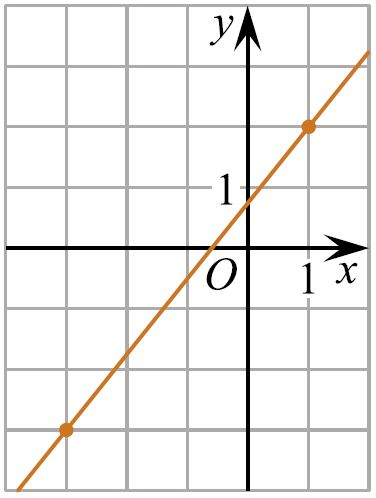
\includegraphics[align=t, width=0.8\textwidth]{../../pics/G112M3C2-1}
		\end{minipage}
		\item
		\begin{minipage}[t]{0.2\textwidth}
			На рисунке изображены графики двух линейных функций. Найдите абсциссу точки пересечения графиков.
		\end{minipage}
		\begin{minipage}[c]{0.2\textwidth}
			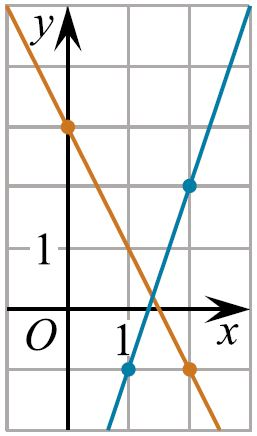
\includegraphics[align=t, width=0.8\textwidth]{../../pics/G112M3C2-2}
		\end{minipage}
		\item
		\begin{minipage}[t]{0.2\textwidth}
			На рисунке изображен график функции \( f(x)=\dfrac{x^2}{a}+bx+c \). Найдите \( f(3,5) \).
		\end{minipage}
		\begin{minipage}[c]{0.2\textwidth}
			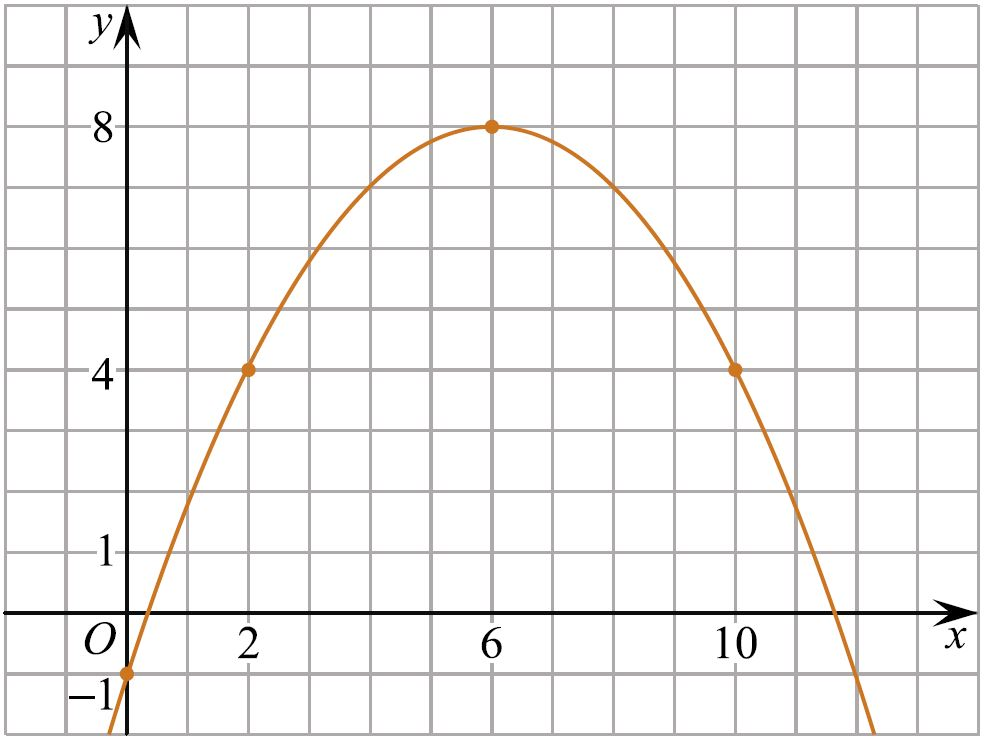
\includegraphics[align=t, width=\textwidth]{../../pics/G112M3C2-3}
		\end{minipage}
		\item
		\begin{minipage}[t]{0.2\textwidth}
			На рисунке изображен график функции \( f(x)=\dfrac{x^2}{a}+bx+c \). Найдите \( f(4) \).
		\end{minipage} 
		\begin{minipage}[c]{0.2\textwidth}
			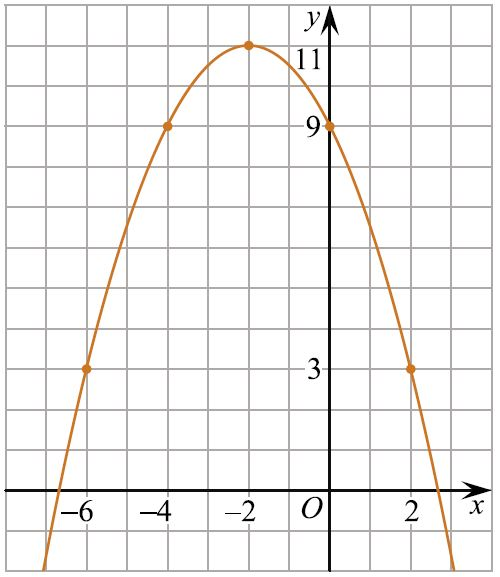
\includegraphics[align=t, width=\textwidth]{../../pics/G112M3C2-4}
		\end{minipage}
		\item Из городов \( A \) и \( B \), расстояние между которыми равно \( 330 \) км, навстречу друг другу одновременно выехали два автомобиля и встретились через \( 3 \) часа на расстоянии \( 180 \) км от города \( B \). Найдите скорость автомобиля, выехавшего из города \( A \). Ответ дайте в км/ч.
		\item Из двух городов, расстояние между которыми равно \( 560 \) км, навстречу друг другу одновременно выехали два автомобиля. Через сколько часов автомобили встретятся, если их скорости равны \( 65 \) км/ч и \( 75 \) км/ч?
		\item Иван и Алексей договорились встретиться в Н-ске. Они едут к Н-ску разными дорогами. Иван звонит Алексею и узнаёт, что тот находится в \( 168 \) км от Н-ска и едет с постоянной скоростью \( 72 \) км/ч. Иван в момент звонка находится в \( 165 \) км от Н-ска и ещё должен по дороге сделать \( 30 \)-минутную остановку. С какой скоростью должен ехать Иван, чтобы прибыть в Н-ск одновременно с Алексеем?
=======
		\item Моторная лодка прошла против течения реки \( 255 \)  км и вернулась в пункт отправления, затратив на обратный путь на \( 2 \)  часа меньше. Найдите скорость лодки в неподвижной воде, если скорость течения равна \( 1 \)  км/ч. Ответ дайте в км/ч.
		\item По морю параллельными курсами в одном направлении следуют два сухогруза: первый длиной \( 120 \)  метров, второй --- длиной \( 80 \)  метров. Сначала второй сухогруз отстает от первого, и в некоторый момент времени расстояние от кормы первого сухогруза до носа второго составляет \( 400  \) метров. Через \( 12 \) минут после этого уже первый сухогруз отстает от второго так, что расстояние от кормы второго сухогруза до носа первого равно \( 600 \)  метрам. На сколько километров в час скорость первого сухогруза меньше скорости второго?
		\item Моторная лодка прошла против течения реки \( 112 \)  км и вернулась в пункт отправления, затратив на обратный путь на \( 6 \)  часов меньше. Найдите скорость течения, если скорость лодки в неподвижной воде равна \( 11 \)  км/ч. Ответ дайте в км/ч
		\item Теплоход проходит по течению реки до пункта назначения \( 255 \)  км и после стоянки возвращается в пункт отправления. Найдите скорость теплохода в неподвижной воде, если скорость течения равна \( 1 \)  км/ч, стоянка длится \( 2 \)  часа, а в пункт отправления теплоход возвращается через \( 34 \)  часа после отплытия из него. Ответ дайте в км/ч.
		\item Моторная лодка в \( 10:00 \)  вышла из пункта \( A \) в пункт \( B \) , расположенный в \( 30 \)  км от \( A \). Пробыв в пункте В \( 2 \)  часа \( 30 \)  минут, лодка отправилась назад и вернулась в пункт \( A \)  в \( 18:00 \) того же дня. Определите (в км/ч) собственную скорость лодки, если известно, что скорость течения реки \( 1 \)  км/ч.
		\item Первый игральный кубик обычный, а на гранях второго кубика нет нечётных чисел, а чётные числа \( 2 \), \( 4 \) и \( 6 \) встречаются по два раза. В остальном кубики одинаковые.Один случайно выбранный кубик бросают два раза. Известно, что в каком-то порядке выпали \( 4 \) и \( 6 \) очков. Какова вероятность того, что бросали первый кубик?
		\item Игральную кость бросили один или несколько раз. Оказалось, что сумма всех выпавших очков равна \( 3 \). Какова вероятность того, что было сделано два броска? Ответ округлите до сотых.
		\item Игральную кость бросили один или несколько раз. Оказалось, что сумма всех выпавших очков равна \( 4 \). Какова вероятность того, что был сделан один бросок? Ответ округлите до сотых.
		\item Стрелок стреляет по одному разу по каждой из пяти одинаковых мишеней. Вероятность поразить мишень каждым отдельным выстрелом равна \( 0,8 \). Во сколько раз вероятность события «стрелок поразит ровно четыре мишени» больше вероятности события «стрелок поразит ровно три мишени»?
		\item В магазине стоят два платёжных автомата. Каждый из них может быть неисправен с вероятностью \( 0,05 \)  независимо от другого автомата. Найдите вероятность того, что хотя бы один автомат исправен.
		\item Всем пациентам с подозрением на гепатит делают анализ крови. Если анализ выявляет гепатит, то результат анализа называется положительным. У больных гепатитом пациентов анализ даёт положительный результат с вероятностью \( 0,9 \). Если пациент не болен гепатитом, то анализ может дать ложный положительный результат с вероятностью \( 0,01 \). Известно, что \( 5\% \) пациентов, поступающих с подозрением на гепатит, действительно больны гепатитом. Найдите вероятность того, что результат анализа у пациента, поступившего в клинику с подозрением на гепатит, будет положительным.		
>>>>>>> cbeab13056f26d5b6e6a0443a5ebe66bd0f83c32
	\end{listofex}
\end{class}
%END_FOLD

%BEGIN_FOLD % ====>>_ Домашняя работа 2 _<<====
\begin{homework}[number=2]
	\begin{listofex}
		\item Теплоход, скорость которого в неподвижной воде равна \( 17 \) км/ч, проходит по течению реки и после стоянки возвращается в исходный пункт. Скорость течения равна \( 2 \) км/ч, стоянка длится \( 6 \) часов, а в исходный пункт теплоход возвращается через \( 40 \) часов после отправления из него. Сколько километров прошёл теплоход за весь рейс?
		\item Первый игральный кубик обычный, а на гранях второго кубика нет чётных чисел, а нечётные числа \( 1 \), \( 3 \) и \( 5 \) встречаются по два раза. В остальном кубики одинаковые. Один случайно выбранный кубик бросают два раза. Известно, что в каком-то порядке выпали \( 3 \) и \( 5 \) очков. Какова вероятность того, что бросали второй кубик?
	\end{listofex}
\end{homework}
%END_FOLD

%BEGIN_FOLD % ====>>_____ Занятие 5 _____<<====
\begin{class}[number=5]
	\begin{listofex}
		\item Занятие 5
	\end{listofex}
	\end{class}
	%END_FOLD
	
	%BEGIN_FOLD % ====>>_____ Занятие 6 _____<<====
	\begin{class}[number=6]
		\begin{listofex}
			\item Занятие 6
		\end{listofex}
	\end{class}
	%END_FOLD
	
	%BEGIN_FOLD % ====>>_ Домашняя работа 3 _<<====
	\begin{homework}[number=3]
		\begin{listofex}
			\item Домашняя работа 3
		\end{listofex}
	\end{homework}
	%END_FOLD
	
	%BEGIN_FOLD % ====>>_____ Занятие 7 _____<<====
	\begin{class}[number=7]
		\title{Подготовка к проверочной}
		\begin{listofex}
			\item Занятие 7
		\end{listofex}
	\end{class}
	%END_FOLD
	
	%BEGIN_FOLD % ====>>_ Проверочная работа _<<====
	\begin{exam}
		\begin{listofex}
			\item Проверочная
		\end{listofex}
	\end{exam}
	%END_FOLD